\documentclass[border=10pt]{standalone}

\usepackage{tikz}
\usepackage{tikzsymbols}
\usetikzlibrary{calc,patterns,shapes.geometric}

\def\centerarc[#1](#2)(#3:#4:#5){\draw[#1] ($(#2)+({#5*cos(#3)},{#5*sin(#3)})$) arc (#3:#4:#5);}

\begin{document}
	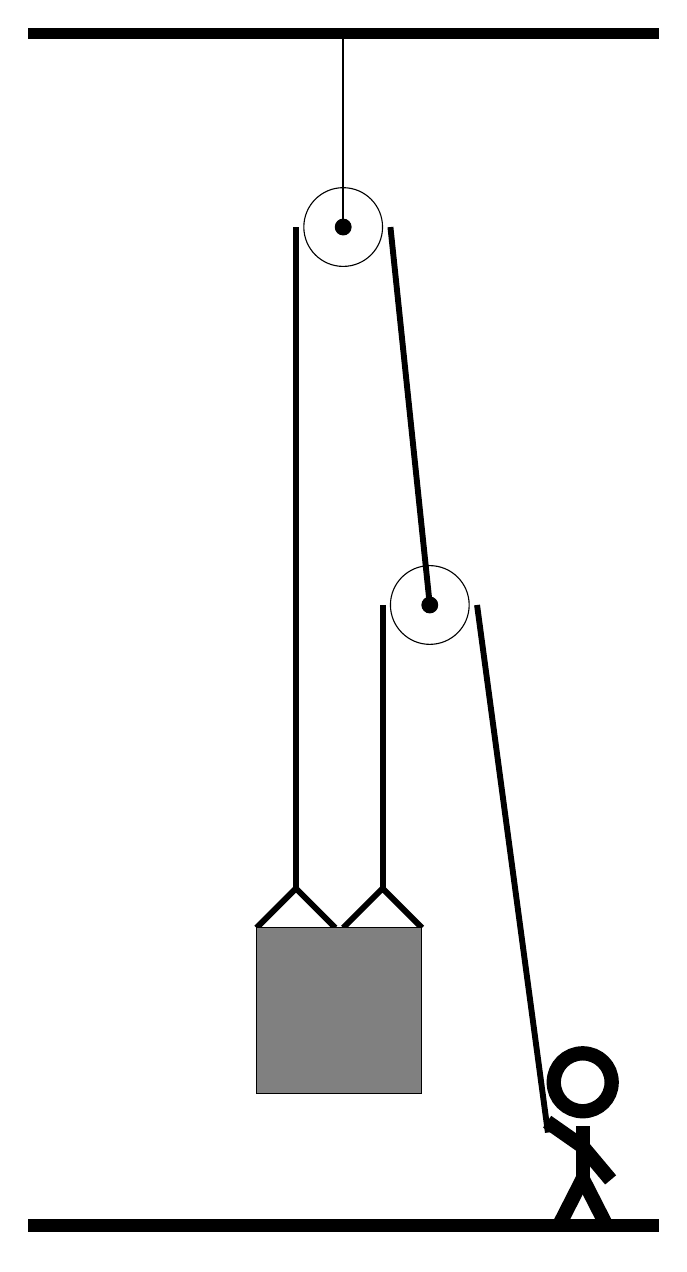
\begin{tikzpicture}
		%%%%% START %%%%%
		\draw[fill=black] (-2, 12) rectangle (6, 12.125);
		
		\draw (2, 9.6) circle (0.5);
		\draw[fill=black] (2, 9.6) circle (0.1);
		\draw[thick] (2, 9.6) -- (2, 12);
		
		\draw (3.1, 4.8) circle (0.5);
		\draw[fill=black] (3.1, 4.8) circle (0.1);
		
		\draw[line width = 0.75mm]  (0.9, 0.7) -- (1.4, 1.2) -- (1.9, 0.7);
		\draw[line width = 0.75mm]  (2.0, 0.7) -- (2.5, 1.2) -- (3.0, 0.7);
		\draw[fill=black!50] (0.9, 0.7) rectangle (3.0, -1.4);
		
		\draw[line width = 0.75mm] (1.4, 9.6) -- (1.4, 1.2);
		\centerarc[line width = 0.75mm](2, 9.6)(0:180:0.6);
		\draw[line width = 0.75mm] (2.6, 9.6) -- (3.1, 4.8);
		\draw[line width = 0.75mm] (2.5, 4.8) -- (2.5, 1.2);
		\centerarc[line width = 0.75mm](3.1, 4.8)(0:180:0.6);
		\draw[line width = 0.75mm] (3.7, 4.8) -- (4.6, -1.9);
		
		\node at (5, -2) {\Strichmaxerl[10][-35][-50]};
		
		\draw[fill=black] (-2, -3) rectangle (6, -3.15);
		%%%%% END %%%%%
	\end{tikzpicture}
\end{document}